\section{Schemes and morphisms (Diego)} % Diego's talk(s)
\label{sec:2_schemes_and_morphisms}
\subsection{Some classical algebraic geometry}
\label{subsec:2_1_classical_AG}
How much can we know about spaces from their functions? A simple example here is the space $\C^n$. Consider the set $R$ of polynomial functions $\C^n \to \C$, which may be identified as $R=\C[x_1, \ldots, x_n]$. Then for each point $p = (p_1, \ldots, p_n) \in \C^n$, we may define the evaluation map $\ev_p : R \to \C$ given by $\ev_p(f) := f(p)$. Clearly this is a surjective morphism of $\C$-algebras, so we can think of this as a map quotienting out by the maximal ideal 
\[
	\mxid_p := \ker(\ev_p) = (x_1-p_1,\ldots,x_n-p_n).
\] 
In fact, all maximal ideals of $R$ are of the form $\mxid_q$ for some $q \in \C^n$, so this defines a bijection
\[
	\begin{tikzcd}[row sep=tiny]
		\C^n \ar[r, leftrightarrow, "\sim"] & \Spec_\mxid(R) \\
		p \rar[mapsto] & \mxid_p 
	\end{tikzcd}
\]
where $\Spec_\mxid(R)$ denotes the \bemph{maximal spectrum} of $R$, that is, the set of maximal ideals of $R$. For each subset $U \subseteq \C^n$ and ideal $J \ideal R$, we may then extend this construction by defining 
\[
	\I(U) := \bigcap_{p \in U} \mxid_p, \quad \text{and} \quad \V(J) := \{p \in \C^n \mid \forall f \in J, \, f(p) = 0 \}.
\]
These two maps end up to be inclusion reversing, and thus define an antitone Galois connection
% https://q.uiver.app/#q=WzAsMixbMCwwLCJcXGxlZnRcXHsgXFxzdWJzdGFja3tcXHRleHR7U3Vic2V0c31cXFxcXFx0ZXh0e29mIH1cXENebn0gXFxyaWdodFxcfSJdLFsyLDAsIlxcbGVmdFxceyAgXFxzdWJzdGFja3tcXHRleHR7SWRlYWxzfSBcXFxcIFxcdGV4dHtvZiB9Un0gXFxyaWdodFxcfSJdLFswLDEsIkkiLDAseyJjdXJ2ZSI6LTJ9XSxbMSwwLCJWIiwwLHsiY3VydmUiOi0yfV1d
\[\begin{tikzcd}
	\begin{array}{c} \left\{ \bettersubstack{\text{Subsets}\\\text{of }\C^n} \right\} \end{array} && \begin{array}{c} \left\{  \bettersubstack{\text{Ideals} \\ \text{of }R} \right\} \end{array}
	\arrow["\I", curve={height=-12pt}, from=1-1, to=1-3]
	\arrow["\V", curve={height=-12pt}, from=1-3, to=1-1]
\end{tikzcd}\]
which restrict to inclusion reversing bijections between the \emph{radical ideals} of $R$ (i.e. those such that if $x^n \in J$ then $x \in J$), and the so-called \emph{algebraic sets} (this is \emph{Hilbert's Nullstellensatz}).

\begin{defn}
	A subset $X \subseteq \C^n$ is called an \bemph{algebraic subset} if it is defined to be the common zero locus of a set of $n$-variable polynomials in $\C^n$.
\end{defn}

We note that:
\begin{itemize}
	\item $\C^n = \V(0)$, so $\C^n$ is an algebraic subset of itself;
	\item $\varnothing = \V(1)$, so $\varnothing$ is an algebraic subset of itself;
	\item as a consequence of \emph{Hilbert's Basis Theorem} (i.e. that $R$ is Noetherian), arbitrary intersections of algebraic subsets are algebraic; and
	\item as a consequence of the fact $\V(f) \cup \V(g) = \V(fg)$, finite unions of algebraic subsets are algebraic.
\end{itemize}
All of these properties say that the algebraic subsets define the closed sets of a topology on $\C^n$, which we call the \bemph{Zariski topology} $\mathcal{T}_\text{Zar}$. That is, a subset of $\C^n$ is Zariski-closed if and only if it is algebraic. 

\begin{defn}
	When $\C^n$ (or equivalently, $k^n$ for a field $k$) is endowed with the Zariski topology $\mathcal{T}_\text{Zar}$, it is referred to as (complex) \bemph{affine $n$-space} $\A^n$. A Zariski closed subset of $\A^n$ endowed with the subspace topology is referred to as a (complex) \bemph{closed affine algebraic variety} (or just a \emph{CAAV}).
\end{defn}

We can check that a basis for the open sets of the Zariski topology is given by open sets of the form
\[
	D_f := \{p \in \A^n \mid f(p) \neq 0\},
\]
which are huge for nonzero polynomials $f\in R$ (cf. Figure \ref{fig:zariski_open})! Because of this, CAAVs are very poorly behaved topological spaces (e.g. they're not Hausdorff), so continuous maps should not necessarily be our notion of a `nice' map. We are usually more interested in polynomial functions on these spaces, which preserve this algebraic structure.

\begin{figure}[H]
	\centering
	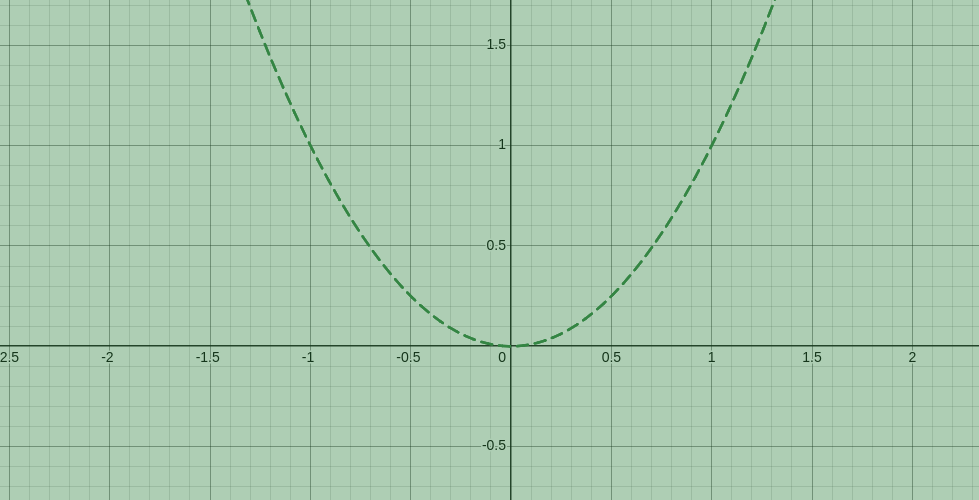
\includegraphics[width=0.5\textwidth]{Images/zariski_open.png}
	\caption{The basic open set $D_{y-x^2}$ in $\A^2$ shaded in light green.}
	\label{fig:zariski_open}
\end{figure}

\begin{eg}
	Let $X = \V(x^2 + y^2 - 1) \subseteq \A^2$ be the circle in the plane\footnote{While we are usually considering things over $\C$, which has topological dimension 2, the algebraic dimension of affine $n$-space is $n$ and so $\A^1$ is referred to as \emph{the line}, $\A^2$ as \emph{the plane}, etc.}. What would the polynomial functions $X \to \A^1$ even be? Well, these should be the restriction of a polynomial function $\A^2 \to \A^1$ to $X$, considered equal if and only if they agree at all points of $X$. The polynomial functions $\A^2 \to \A^1$ are just 2-variable complex polynomials, $\C[x,y]$, and two polynomials $f, g \in \C[x,y]$ agree on $X$ if and only their difference $f-g$ is zero on $X$. The polynomials which are zero on $X$, by definition, are the elements of the vanishing ideal $\I(X) = (x^2 + y^2 - 1)$, and so the polynomial functions $X \to \A^1$ may be identified with elements of the quotient $\C[x, y]/(x^2 + y^2 - 1)$.
\end{eg}

\begin{defn}
	For a closed affine algebraic variety $X \subseteq \A^n$, its \bemph{coordinate ring} $\ints(X)$ is the ring of polynomial functions $X \to \A^1$, that is, it is the quotient ring 
	\[
		\ints(X) := \frac{\C[x_1,\ldots,x_n]}{\I(X)}.
	\]
\end{defn}

We note a few things about coordinate rings of CAAVs over $\C$:
\begin{itemize}
	\item the coordinate ring $\ints(X)$ is a $\C$-algebra, since constant functions are polynomial;
	\item since $\I(X)$ is radical and $\C[x_1, \ldots, x_n]$ is an ID, the quotient $\ints(X)$ is \emph{reduced} (it has no nilpotents);
	\item since $\C[x_1, \ldots, x_n]$ is Noetherian and finitely-generated as a $\C$-algebra, $\ints(X)$ is finitely-generated as a $\C$-algebra.
\end{itemize}

This association of a coordinate ring to each CAAV over $\C$ may be seen to give an equivalence of categories
\[
	\begin{tikzcd}
		\left\{\bettersubstack{\text{closed, affine,} \\ \text{algebraic varieties} \\ \text{over }\C}\right\} \rar[leftrightarrow, "\simeq"] & \left\{\bettersubstack{\text{finitely generated,}\\ \text{reduced, commutative} \\ \C\text{-algebras}}\right\}^{\text{op}}
	\end{tikzcd}
\]
The fully-faithful property is pretty easy to see (our morphisms of CAAVs are just polynomial maps), but the essential surjectivity on objects is a bit more tricky. To show this we think back to the observation that at the beginning of the chapter that points of $\A^n$ are in bijection with maximal ideals of $\C[x_1, \ldots, x_n]$.\\ 

It is not too hard to show that this also holds of any complex CAAV $X$: that points of $X$ are in bijection with maximal ideals of $\ints(X)$. So if we endow $\Spec_\mxid(\ints(X))$ with the Zariski topology, we can view the maximal spectrum \emph{itself} as a CAAV.\\ 

To do this we only need to recall that the evaluation map $\ev_p$ may be seen as the quotient by $\mxid_p$, so the `evaluation' of a `function' $f \in \ints(X)$ at a `point' $\mxid_1 \in \Spec_\mxid(\ints(X))$ is defined to be the residue class $f \mod{\mxid}$. Translating the definition of the basic open sets of $X$ into this language, a basis for the Zariski topology on $\Spec_\mxid (\ints(X))$ is given by the sets of the form 
\[
	D_f := \{ \mxid_1 \in \Spec_\mxid(\ints(X)) \mid f \notin \mxid_1 \}.
\]
Given a finitely generated, reduced, commutative $\C$-algebra $A$, its maximal spectrum $\Spec_\mxid(A)$ under the Zariski topology may then be seen as a closed affine algebraic variety over $\C$ whose coordinate ring is $A$, giving essential surjectivity. To repeat, 
\begin{center}
	a closed affine algebraic variety $X$ \textbf{is} the maximal\\spectrum of its coordinate ring $\ints(X)$:
	\[
		X = \Spec_\mxid(\ints(X))
	\]
\end{center}
As for why this is functorial, the morphism of CAAVs corresponding to an algebra homomorphism $\varphi : A \to B$ is 
\[
	\Spec_\mxid(\varphi) : \Spec_\mxid(B) \to \Spec_\mxid(A), \qquad \mxid_B \mapsto  \phi^{-1}(\mxid_B).
\]


\subsubsection{Why move to schemes?}
\label{subsubsec:2_1_1_why_schemes}
\begin{itemize}
	\item We want to create a similar theory that accepts \emph{any} commutative ring, rather than exclusively finitely generated, reduced, commutative $\C$-algebras;
	\item Since algebraic subsets correspond to radical ideals, this theory does not see points with multiplicity/rings with nilpotence. For example, the equation $x^2 =0$ in $\A^1$ should correspond to a point at zero \emph{with multiplicity 2}, but $\V(x^2) = \V(\sqrt{(x^2)}) = \V(x)$ which only sees that there is a point at zero and forgets the multiplicity;
	\item While $\Spec_\mxid$ is functorial for our FGRC $\C$-algebras, it fails to be functorial in general (preimages of maximal ideals under general ring homomorphisms are rarely maximal, e.g. $(0)$ in $\Z \to \Q$). 
\end{itemize}

\subsection{Affine schemes}
\label{subsec:2_2_affine_schemes}
In much the same way that the theory of varieties revolves around the maximal spectrum, the theory of schemes is based on the \bemph{spectrum} of a commutative ring $R$. This is the set of \emph{prime} ideals of $R$, which we also endow with the Zariski topology 
\[
	\Spec(R) = \{\prid \ideal R \ \text{prime}\}, \qquad D_f = \{\prid \in \Spec(R) \mid f \notin \prid\}, \qquad \mathcal{T}_\text{Zar} = \gen{D_f \mid f \in R}.
\]

For simplicity, we will assume from now on that all rings $R$ are integral domains unless otherwise specified, but bear in mind that all of this can be done over non-integral domains (the definition of localisation does change in this case though).

\begin{defn}
	An \bemph{affine scheme} is a pair $(X, \ints_X)$, where $X = \Spec(R)$ for some commutative ring $R$, and $\ints_X$ is a sheaf\footnote{If you don't know what a sheaf is, I've included \hyperref[appendix:A_sheaves]{a short appendix} on everything you'll need to know about them.} on $X$ (called the \bemph{structure sheaf}) defined on the basic Zariski-open sets $D_f$ to be the localisation of $R$ at $f$
	\[
		\ints_X (D_f) := R_f = R\left[\frac{1}{f}\right],
	\]
	i.e. those elements of the field of fractions $\Frac(R)$ of the form $g / f^n$, where $g \in R$ and $n \in \Z$. The restriction morphisms $\res:\ints_X(D_f) \to \ints_X(D_{fg})$ is the usual inclusion map.
\end{defn}

We can check that the stalks of $\ints_X$ are given by
\[
	\ints_{X, \prid} = \varinjlim_{U \ni \prid} \ints_X(U) = R_\prid,
\]
the localisation of $R$ at $\prid$, i.e. those elements of $\Frac(R)$ whose denominator is not in $\prid$. Since $R_{\prid}$ is local, affine schemes are locally ringed spaces. If a locally ringed space $(X, \ints)$ is isomorphic to an affine scheme, we will call it an affine scheme also.\\

As before, for each $\prid \in \Spec(R)$ we define the \bemph{evaluation map} $\ev_\prid$ to be the quotient map with kernel $\prid$, although now it is valued in the \bemph{residue field} $k(\prid) := \Frac(R/\prid) = R_\prid / \prid R_\prid$. This allows us to define our $\V$ and $\I$ functions as before:
\begin{align*}
	\V(J) &:= \{\prid \in \Spec(R) \mid \ev_\prid(f)=0, \ \forall f \in J\} = \{\prid \in \Spec(R) \mid J \subseteq \prid\},\\
	\I(U) &:= \{f \in R \mid \ev_\prid(f) = 0, \ \forall \prid \in U\} = \bigcap_{\prid \in U} \prid,
\end{align*}
where $J\ideal R$ is an ideal and $U \subseteq \Spec(R)$ is a subset. Notably, we see that:
\begin{itemize}
	\item the Zariski-closure $\ol{U}$ of a subset $U \subseteq \Spec(R)$ is exactly $\ol{U} = \V\I(U)$;
	\item the correspondence theorem ensures that $\V(J) \subseteq \Spec(R)$ may be identified with the affine scheme $\Spec(R/J)$, so the Zariski-closed subsets are the spectra of quotients of $R$ (and $\varnothing$);
	\item properties of localisation ensure that $D_f \subseteq \Spec(R)$ may be identified with the affine scheme $\Spec(R_f)$, so the basic Zariski-open subsets are the spectra of localisations of $R$.
\end{itemize}

\begin{eg}
	\begin{enumerate}[(i)]
		\item While we have seen that the closed affine algebraic variety $\Spec_\mxid(\C[x,y])$ may be identified with $\C^n$ under the Zariski topology, we instead look at the prime spectrum $\Spec(\C[x,y])$. As a set, this decomposes as 
			\[
				\Spec(\C[x,y]) = \Spec_\mxid (\C[x,y]) \,\, \cup \,\, \{(0)\} \,\, \cup \,\, \{(f) \mid f \in \C[x,y] \text{ irr.}\}.
			\]
			These different categories of points are distinguished by the Zariski closures of their corresponding singletons, which is exactly $\V\I(\{\prid\})=\V(\prid)$.
			\begin{itemize}
				\item For a point $\mxid_1 \in \Spec_\mxid(\C[x,y])$, i.e. a maximal ideal of $\C[x,y]$, we see that $\ol{\{\mxid_1\}} = \V(\mxid_1)$ is the set of prime ideals containing $\mxid_1$, which is exactly the singleton $\{\mxid_1\}$ since $\mxid_1$ is maximal. For this reason, maximal ideals of $\C[x,y]$ correspond to \bemph{closed points} of $\Spec(\C[x,y])$ (and this works for general rings!);
				\item The point $(0) \in \Spec(\C[x,y])$, i.e. the zero ideal, has $\ol{\{(0)\}} = \V(0) = \Spec(\C[x,y])$. For this reason, the point $(0)$ is called a \bemph{dense point} or a \bemph{generic point} of $\Spec(\C[x,y])$ (and again, this works for general rings);
				\item A point $(f) \in \Spec(\C[x,y])$ with $f \in \C[x,y]$ irreducible has $\ol{\{(f)\}} = \V(f) = \Spec(R/(f))$, which is a closed affine subscheme (i.e. a Zariski closed subset). Such points are thus the generic points of closed affine subschemes of $\Spec(\C[x,y])$.
			\end{itemize}
			So the points of $\Spec(\C[x,y])$ may be thought of as
			\[
				\Spec(\C[x,y]) = \left\{\bettersubstack{\text{closed} \\ \text{points}}\right\} \,\, \cup \,\, \left\{\bettersubstack{\text{generic} \\ \text{point}}\right\} \,\, \cup \,\, \left\{\bettersubstack{\text{generic points of} \\ \text{closed subschemes}}\right\}
			\]
			We may think of generic points as a sort of `codimension 0 point', which is close to everything. 
		\item The affine scheme $\Spec(\C[x]/(x^2))$ decomposes as
			\[
				\Spec\left(\frac{\C[x]}{(x^2)}\right) = \{(x)\} \,\,\cup\,\, \{(0)\}
			\]
			which is just the one closed point, along with the generic point. This is seen to be different to $\Spec(\C[x]/(x)) = \Spec(\C)$, which consists solely of a generic point. So our notion is tracking multiplicity correctly!
		\item One interesting example that may motivate something later: if we consider the prime spectrum of $\Z$, this may be visualised as a long line (corresponding to the generic point) connecting infinitely many points (corresponding to the closed points, the ideals $p\Z$), as in Figure \ref{fig:SpecZ}.
		\begin{figure}[H]
			\centering
			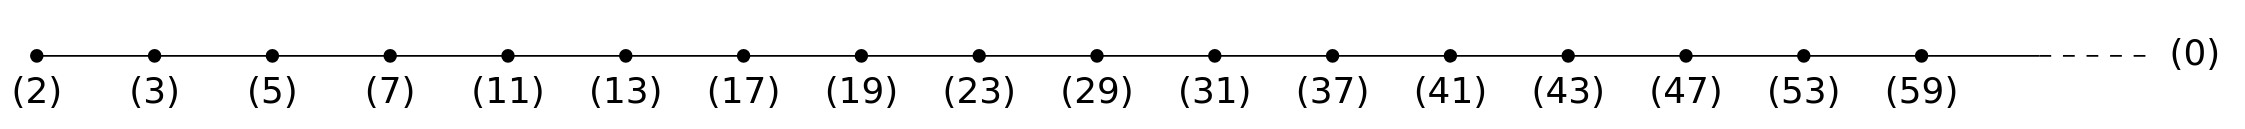
\includegraphics[width=0.7\textwidth]{Images/Spec(Z).png}
			\caption{$\Spec(\Z)$, per the \href{https://www.lmfdb.org/NumberField/1.1.1.1}{LMFDB}.}
			\label{fig:SpecZ}
		\end{figure}
		The inclusion $\Z \mono \Z[\!\sqrt{3}]$ gives us a corresponding surjective morphism $\Spec(\!\Z[\sqrt{3}]) \epi \Spec(\Z)$ which may be visualised as in Figure \ref{fig:SpecZsqrt3_over_SpecZ}, where the vertical columns are the fibres of the morphism.
		\begin{figure}[H]
			\centering
			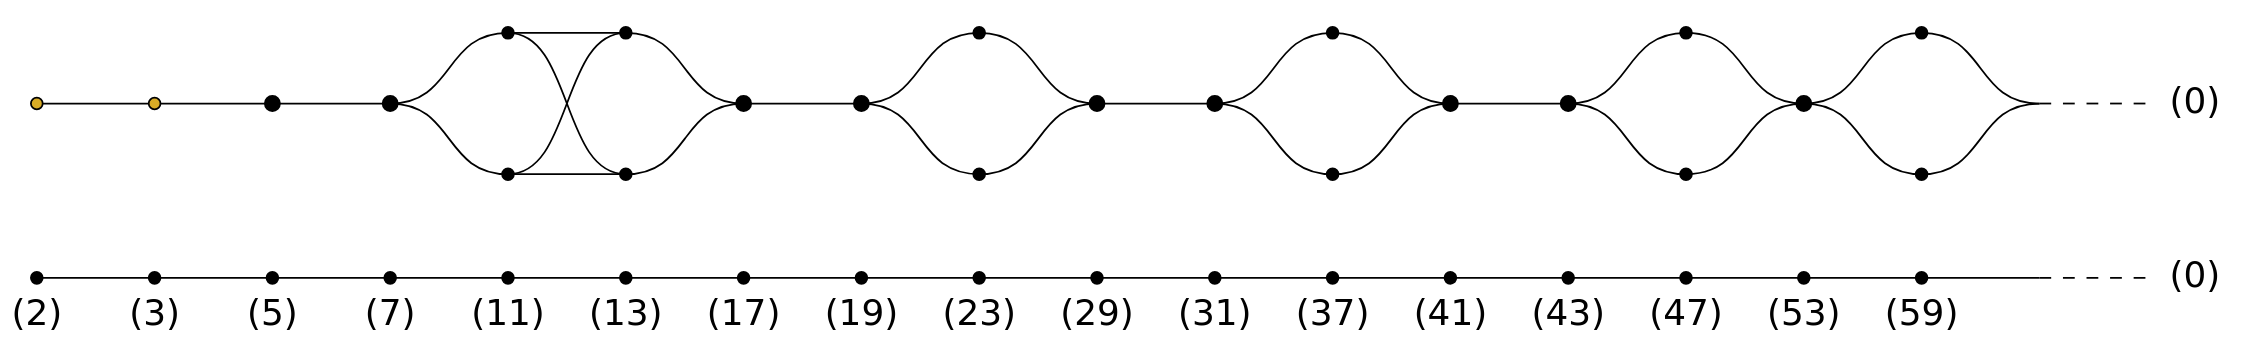
\includegraphics[width=0.7\textwidth]{Images/ramification_diagram_Zsqrt3.png}
			\caption{$\Spec(\Z[\!\sqrt{3}])\epi\Spec(\Z)$, per the \href{https://www.lmfdb.org/NumberField/2.2.12.1}{LMFDB}.}
			\label{fig:SpecZsqrt3_over_SpecZ}
		\end{figure}
		The behaviour of different points fall into three classes, all depicted differently in this diagram:
		\begin{itemize}
			\item \textbf{A single, black point} above a point $(p)$ of $\Spec(\Z)$ corresponds to the ideal $p\Z[\!\sqrt{3}]$ being a prime ideal of $\Z[\sqrt{3}]$, as we see with e.g. $(17)$. This point $17\Z[\!\sqrt{3}]$ of $\Spec(\Z[\!\sqrt{3}])$ is a \bemph{reduced point}, i.e. a point with multiplicity 1. In the number theory lingo, we say that $17$ is \bemph{inert} in the extension $\Q(\!\sqrt{3})/\Q$;
			\item \textbf{Two different black points} above a point $(p)$ of $\Spec(\Z)$ corresponds to the ideal $p\Z[\!\sqrt{3}]$ decomposing as a product of two distinct prime ideals $\Prid_1, \Prid_2$ in $\Z[\sqrt{3}]$ each with multiplicity 1, as we see with e.g. $(11)$ decomposing in $\Z[\!\sqrt{3}]$ as $(1-2\sqrt{3})(1+2\sqrt{3})$. Both of these points $\Prid_1, \Prid_2$ above $(p)$ are again reduced points of $\Spec(\Z[\!\sqrt{3}])$. In the number theory lingo, we say that $11$ is \bemph{completely split} in $\Q(\!\sqrt{3})/\Q$, and we say that $(1-2\sqrt{3})$ and $(1+2\sqrt{3})$ are the primes \bemph{above} $11$;
			\item \textbf{A single, yellow point} above a point $(p)$ of $\Spec(\Z)$ corresponds to the ideal $p\Z[\!\sqrt{3}]$ being the square\footnote{...or more generally, a power of a single prime ideal.} of a single prime ideal $\Prid$ in $\Z[\!\sqrt{3}]$, as we see with e.g. $3\Z[\!\sqrt{3}] = (\sqrt{3})^2$. This point $(\sqrt{3})$ is a \bemph{non-reduced point} of multiplicity 2. In the number theory lingo, we see that $3$ is \bemph{totally ramified} in $\Q(\!\sqrt{3})/\Q$, and we say that $(\sqrt{3})$ is the prime above $3$.
		\end{itemize}
	\end{enumerate}
\end{eg}




% talk about Diego's ramification intuition in the morphisms-y bit